\section{Problema 2: Reconfiguraci\'on de rutas}

\subsection{Introducci\'on}

\quad Se desea optimizar las conexiones existentes entre un conjunto de ciudades. Se pueden construir nuevos caminos o destruir existentes. Ambas operaciones tienen un costo asociado. Se desea optimizar gastando la menor cantidad de dinero posible. Solo puede haber una forma de ir de una ciudad a otra y no existen varias rutas entre dos mismas ciudades. Bajo estas premisas resolvimos el problema como detallaremos a continuación.


\subsection{Desarrollo}

\quad Decidimos modelar el problema con grafos. Donde, los nodos son las ciudades y las aristas son las rutas existentes y las posibles a construir. Cada eje tiene un costo asociado, ya sea para destruir o construir la ruta que simboliza. Destacamos el hecho de que las instancias del problema por consigna tienen $ \frac{n * (n - 1)}{2} $ aristas donde $ n $ es la cantidad de ciudades. Por la propiedad de grafos vista en la cursada, esa es la cantidad de aristas que tienen los grafos completos de $ n $ nodos. Por lo tanto, siempre como entrada al problema, se reciben grafos completos de $ n $ nodos.

\quad

\quad Luego, utilizamos el algoritmo modificado de Kruskal para generar un \'arbol generador m\'inimo (AGM) del grafo. A diferencia de realizar normalmente este algoritmo, utilizamos un ordenamiento de las aristas distinto. Primero consideramos como menores todas las aristas de rutas ya construidas que las no existentes. Luegos, las existentes las ordenamos de mayor a menor según el valor asociado. En cambio, las no construidas las ordenamos de menor a mayor. En la parte de correctitud explicaremos el motivo de tal ordenamiento. Podemos resolver el problema con un AGM pues cada ruta es doble vía, se quiere que todas las ciudades est\'en conectadas y que haya una sola forma de ir de una ciudad a otra.

\quad

\quad Para generar el AGM utilizamos una estructuras de datos llamada \textit{Find Union Set} o \textit{Disjoint Set} \footnote{UnionFind Set, Introduction to Algorithms 2nd Edition, Capitulo 21. Autores: Thomas H. Cormen, Charles E. Leiserson, Ronald L, Rivest, Clifford Stein} . Nos permite tener informaci\'on de elementos particionados en clases de equivalencia. Es decir, podemos manejar particiones disjuntas de un conjunto. En este caso, el conjunto de nodos. Las particiones ser\'ian los nodos que pertenecen a una componente conexa. La relaci\'on de clase de equivalencia ser\'ia que exista un camino entre los elementos (nodos) de la clase. En el algoritmo de Kruskal, nos permite determinar si se agregase cierta arista se forma o no un ciclo.

\quad 


\begin{figure}[H]
	\centering
	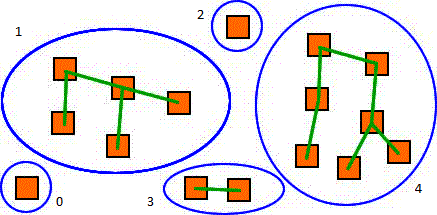
\includegraphics[scale=0.8]{DisjointSets.png}
\caption{Disjoint Set donde hay 5 clases de equivalencia. Los cuadrados naranjas representan nodos y las l\'ineas verdes aristas. Se observa que la relaci\'on es que est\'en en la misma componente conexa.}
\end{figure}



\quad Una vez obtenido el AGM, para calcular el costo de la optimizaci\'on de la conectividad entre las ciudades, es cuesti\'on de recorrer el AGM primero fijándose las aristas que est\'an presentes. Si son aristas de rutas ya existentes no aportan al costo, y si son aristas de rutas nuevas se acumula al costo su valor asociado. Luego, se recorre el grafo original. Se ignoran las aristas de rutas nuevas pero para las aristas de rutas existentes nos fijamos si se encuentran en el AGM. En caso de no estar presente, su valor asociado se suma al acumulador de costo de optimizaci\'on.

\quad 

\quad Como resultado, se devuelve el costo total, la cantidad de aristas del AGM (que siempre va a ser la cantidad de ciudades menos uno al ser un \'arbol) y las aristas pertenecientes al AGM sin su valor asociado.

\subsubsection{Correctitud}

\quad Para ver que se resuelve correctamente el programa con lo implementado, hay que ver la correctitud del modelado del problema con grafos, del algoritmo de Kruskal y que el criterio de ordenamiento elegido es correcto.

\begin{itemize}


\item \textbf{Modelado y criterio de ordenamiento}

\quad Al buscar que entre las ciudades se pueda ir de una \'unica forma, es equivalente a que haya un \'unico camino simple entre nodos de un \'arbol.  Mantener rutas existentes no representan ningún coste, por lo cual uno de nuestros objetivos es mantener la mayor cantidad posible de rutas existentes siempre y cuando no formen un ciclo. De ahí el criterio de que para construir el AGM con Kruskal, las rutas existentes son consideradas menores que las rutas posibles a construir y además, se las ordena de mayor costo a menor pues para darle prioridad de pertenecer al AGM a las que cuestan más destruirlas. En cambio, las no existentes se las ordena de menor a mayor, porque dado el caso de tener que construir nuevas rutas, tengan prioridad las que cuesten menos.

\quad

\quad

\item \textbf{Kruskal}

\quad Extra\'ido de las diapositivas de la clase te\'orica de la materia\footnote{Clase teórica de Árboles, Algoritmos y Estructuras de Datos III, 1er Cuatrimestre 2012, Departamento de Computación, Facultad de Ciencias Exactas y Naturales, UBA http://www-2.dc.uba.ar/materias/aed3/2012-01/Documents/algo3\_arboles\_2012\_handout.pdf}:

\begin{quotation}
 

\quad Se parte de un subgrafo generador cuyo conjunto de aristas es vac\'io, y en cada paso se agrega una arista de peso m\'inimo que no forme ciclos con 
las dem\'as aristas del conjunto, hasta haber agregado $n - 1$ aristas.

\quad Para ver que el algoritmo construye un \'arbol generador, como en cada paso el subgrafo \textit{B} elegido hasta el momento es generador y ac\'iclico,
basta ver que el algoritmo termina con $ m_B  =  n_G - 1$. Si $ m_B < n_G - 1$, B es no conexo. Sea $ B_1 $ una componente conexa de \textit{B}. Como \textit{G} es conexo, va a existir alguna arista con un extremo en $ B_1 $ y el otro en $ V(G) - B_1 $, por lo tanto no forma ciclo con las dem\'as aristas de \textit{B}. Entonces, si $ m_B < n_G - 1$, el algoritmo puede realizar un paso m\'as.

\quad Sea G un grafo, $ T_k $ el \'arbol generado por el algoritmo de \textit{Kruskal} y $ \lbrace e_1, e_2, ..., e_{n-1} \rbrace $ la secuencia de aristas de $ T_k $ en el orden en que fueron elegidas por el algoritmo de \textit{Kruskal}. Para cada \'arbol generador de \textit{T} de \textit{G} definimos $\ell($ \textit{T} $)$ como el m\'aximo $ k \leq n $ tal que $ \forall j < k $, $ e_j \epsilon $ \textit{T}.

\quad Ahora sea T un \textit{AGM} que maximiza \textit{p}. Si $\ell($ \textit{T} $) = n $, entonces \textit{T} coincide con $ T_k $, con lo cual $ T_k $ resulta ser m\'inimo. Si $ T_k $ no es m\'inimo, entonces $\ell($ \textit{T} $) < n $ y $ e_{\ell(T)} \notin T $. Como \textit{T} es conexo, en \textit{T} hay un camino \textit{C} que une los extremos de $ e_{\ell(T)} $.

\quad Como $ T_k $ es ac\'iclico, hay alguna arista \textit{e} en \textit{C} tal que $ e\notin T_k $. Como $ e_1, ..., e_{\ell(T) - 1} \in T $ y \textit{T} es ac\'iclico, \textit{e} no forma ciclos con $ e_1, ..., e_{\ell(T) - 1} $.
Por la forma en que fue elegida $ e_{\ell(T)} $ por el algoritmo de Kruskal, \textit{peso}($e_{\ell(T)}$) $ \leq $ \textit{peso}(\textit{e}).
Pero entonces, $ T' = T - e \cup \lbrace e_{\ell(T)} \rbrace $ es un \'arbol generador de \textit{G} de peso menor o igual a \textit{T} y $ \ell(T') > \ell(T)$, absurdo.

\quad Luego $ T_k $ es un \'arbol generador m\'inimo.

\end{quotation} 

\end{itemize}

\subsubsection{An\'alisis de complejidad}

\quad Implementamos una clase \textit{Grafo}, la cual tiene internamente una variable entera que almacena la cantidad de nodos presentes en el grafo y las aristas en un vector de elementos del tipo \textit{Camino}. 

\quad

\quad Esta clase \textit{Camino} la creamos con el objetivo de hacer m\'as legible el c\'odigo. Es un \textit{wrapper} para una tupla de la siguiente forma: 

\quad

$ \langle Natural Ciudad1, Natural Ciudad2, Booleano Existente, Natural Costo \rangle$

\quad 

\quad Donde \textit{Ciudad1} es el id del nodo que simboliza ese n\'umero de ciudad, an\'alogo con \textit{Ciudad2}. El booleano \textit{Existente}, determina si es una ruta nueva o ya presente en esquema de conexi\'on entre las ciudades. Costo es dependiente del valor del booleano, si es de construcci\'on o destruicci\'on. Tiene operaciones de costo constante ya que son solo asignaciones o obtenci\'on de valor de variables enteras. Adem\'as, y lo fundamental para minimizar el costo de reformar las conexiones de las ciudades, es que se define el operador $ < $ para las aristas del tipo \textit{Camino}. Se defini\'o bajo el criterio anteriormente explicado en la secci\'on de correctitud.

\quad

\quad Se implementa la clase \textit{DisjointSet} mencionada anteriormente. El constructor de la clase toma como un par\'ametro un entero x para crear x particiones. Internamente usa un vector de enteros que recorre asignando a cada posici\'on el valor del \'indice. Tiene costo O($ x $).

\quad La funci\'on \textit{buscar()}, dado dos n\'umeros de nodos se fija en el \textit{vector} si tienen el mismo identificador de clase. De ser as\'i, entonces pertenecen a la misma clase. Es decir, que los nodos est\'an conectados, existe un camino entre esos nodos, lo cual, agregar una arista que una 
directamente esos nodos generar\'ia un ciclo. Al ser un vector, acceder a un elemento es costo constante, entonces \textit{buscar()} es \textit{O($ 1 $)}.

\quad La funci\'on \textit{unir()}, dado dos identificadores de nodo, une ambas clases de esos nodos. Como se dijo anteriormente, se elige un identificador de clase de alguno de los dos nodos y a la otra se le reemplaza su identificador por este. Para esto, se recorren todos los nodos del grafo y adentro del ciclo se usan funciones con costo \textit{O($ 1 $)}, por lo tanto \textit{unir()} cuesta \textit{O($ \sharp nodos $)}. 

\quad

\quad La clase \textit{Grafo} tiene las siguientes operaciones:

\begin{itemize}
\item \textbf{Constructor($ \sharp nodos $):} Se guarda la cantidad de nodos y se reserva espacio suficiente para evitar realocaci\'on de memoria. O($ \sharp nodos^{2} $). Cabe destacar que no contiene aristas.


\item \textbf{agregarArista(Camino c):} Se agrega al vector de aristas una copia del elemento c. O($ 1 $)

\item \textbf{getNodos():} Devuelve la cantidad de nodos del grafo. O($ 1 $)

\item \textbf{AGM():} devuelve un grafo generador m\'inimo del grafo en cuesti\'on. 

\begin{algorithm}[H]
\begin{algorithmic}[1]
\STATE Grafo res(getNodos(ciudades))
\STATE DisjointSet ds(getNodos(ciudades))
\STATE Vector caminos  \quad $ \leftarrow $ \quad aristas(ciudades)
\STATE Sort(caminos)
\FORALL{ Camino c \textbf{in} caminos}
\IF{not buscar(ds,getCiudad1(c),getCiudad2(c))}
\STATE agregarArista(res,c)
\STATE unir(ds,getCiudad1(c),getCiudad2(c))
\ENDIF
\IF{cantAristas(res) = getNodos(ciudades) -1}
\STATE \textbf{exit \textit{for}}
\ENDIF
\ENDFOR
\STATE \textbf{return} res
\end{algorithmic}
\caption{Grafo AGM(Grafo ciudades)}\label{AGM}
\end{algorithm}


\quad Primero crea un grafo que se va a devolver como resultado con la misma cantidad de nodos que el grafo \textit{ciudades} con costo O($ \sharp nodos $). Este grafo no contiene aristas. Luego, se crea un objeto del tipo \textit{DisjointSet} para mantener un registro de las particiones, que como se dijo anteriormente, evita que formemos ciclos. \'Esto tiene costo de O($\sharp nodos^{2}$).

\quad En la siguiente l\'inea, se copia por comodidad las aristas del grafo a un vector (O($\sharp nodos$)), y se las ordena según el criterio definido en la clase \textit{Camino}. Se utiliza la funci\'on \textit{Sort} de la \textit{standard library de C++} por lo que tiene un costo de O($\sharp nodos \ast log(\sharp nodos) $). \quad \footnote{http://www.sgi.com/tech/stl/sort.html}

\quad Una vez ordenadas las aristas, se las recorre. Para cada una, se usa la funci\'on \textit{buscar()} de la clase \textit{DisjointSet} con costo O($ 1 $). En caso de que devuelva verdadero, significa que ya existe un camino entre esas ciudades por lo que agregar esa arista generar\'ia un ciclo. Caso contrario, se agrega la arista al grafo resultado (O($ 1 $)) y se actualiza la informaci\'on de \textit{ds} usando \textit{unir()} con costo O($ \sharp nodos $). 

\quad Se agrega un punto de corte al \textit{for} aprovechando la propieda de \'arboles de que la cantidad de aristas es igual a la cantidad de nodos menos uno y queremos que el grafo resultado sea un AGM.

\quad

\quad En el peor caso, el bucle \textit{for} va a recorrer todas las aristas del grafo original. Al ser un grafo completo son $ \frac{n * (n - 1)}{2} $ iteraciones. Pero, solamente $ n-1 $ iteraciones se va a llamar a la funci\'on \textit{unir()} y el resto de las iteraciones hace operaciones con costo constante. Por lo que la complejidad del ciclo termina siendo:

\quad 

 O($ Max\lbrace (n-1)\ast n, [\frac{n * (n - 1)}{2} - (n-1)] \ast 1 \rbrace $)

\quad

Por lo que es igual a:

\quad

O($ Max\lbrace n^2, n^2 \rbrace $) = O($ n^2 $)

\quad

\quad Por lo que la complejidad de AGM es O($ n +  n \ast log(n) + n^2$) = O($ n^2 $)

\quad Esta complejidad es menor a la requerida: O($ n^{2} \ast log(n)$)

\quad Donde $ n $ es la cantidad de nodos.

\end{itemize}


\subsection{Resultados}

\quad Para poder testear nuestra soluci\'on, decidimos generar grafos completos, donde aleatoriamente se eleg\'ia si una arista era un camino existente o no, y el costo un n\'umero arbitrariamente entre 500 y 10500. 

\quad

\quad Vemos dos casos donde hay pocas aristas de caminos existentes y otro donde hay una mayor cantidad. Ambos casos, se va a ir variando la cantidad de nodos desde 4 hasta 200 con 50 repeticiones por cantidad. Y adem\'as, separamos la implementaci\'on en con y sin punto de corte, del cual se habló anteriormente.

\quad

\quad Las gr\'aficas que nos quedaron son:

\quad

\begin{figure}[H]
	\centering
	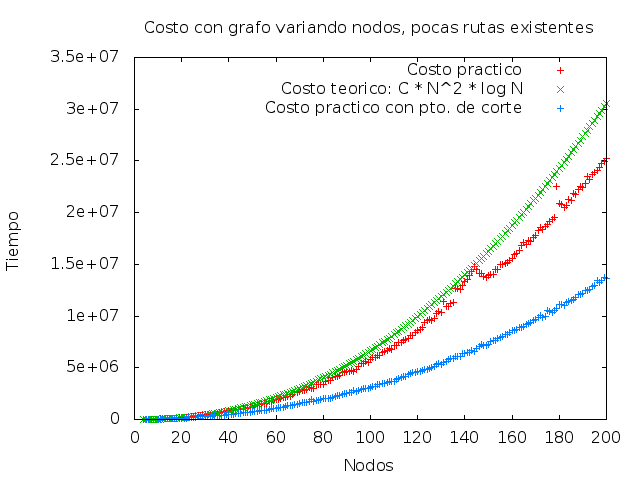
\includegraphics[scale=0.6]{ej2-grafico1.png}
\end{figure}


\begin{figure}[H]
	\centering
	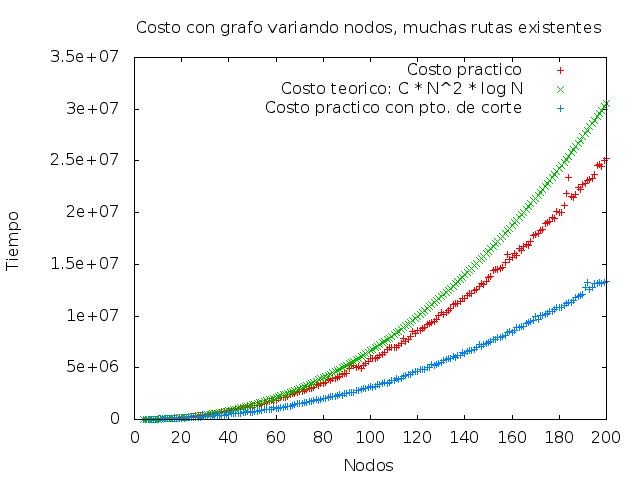
\includegraphics[scale=0.6]{ej2-grafico2.png}
\end{figure}

\quad Se observa como todos los datos obtenidos emp\'iricamente a partir de cierto puento est\'an por debajo de la cota te\'orica. 

\quad

\quad En el c\'odigo del programa, hay una define \textit{TESTING}, que al setearlo en 1 el programa gener\'a los casos de tests nada más. Debido a que se usan grafos completos, y usar una cantidad considerable de nodos y repeciciones se genera un archivo de test bastante pesado. Por lo que no se entrega con este trabajo aunque est\'a la posibilidad de generarlo. Sin comprimir son 1.8 GB, comprimido 600 MB.

\quad 

\subsection{Conclusiones}

\quad Con este tipo de problemas podemos ver la importancia de algunas estructuras de datos no tan comunes pero que facilitan considerablemente la realizaci\'on de alg\'un algoritmo. En este caso, la estructura \textit{DisjointSet} evita que recorramos el grafo fij\'andonos si agregando cierta arista se produce un ciclo en el mismo.

\quad Tambi\'en como, analizando el problema y propiedades de la soluci\'on del mismo, se pueden llegar a encontrar puntos de corte. Si bien pueden no llegar a mejorar la complejidad asint\'otica, como en este caso, mejoran considerablemente en la pr\'actica. En este caso, fue el corte de que la cantidad de aristas  de un \'arbol es igual a la cantidad de nodos menos uno.
